\documentclass[11pt]{article}
\setlength{\parindent}{10pt}
\usepackage [square,colon]{natbib}
\usepackage[utf8]{inputenc}
\usepackage[british]{babel}
\usepackage {comment}
\usepackage[flushleft]{threeparttable}
\renewcommand{\familydefault}{\sfdefault}
\usepackage[a4paper, margin=1.5cm]{geometry}
\usepackage{doi}
\usepackage{subcaption}
\renewcommand{\rmdefault}{phv} % Arial
\renewcommand{\sfdefault}{phv} % Arial
\usepackage[modulo]{lineno}
\usepackage{array}
\newcolumntype{L}[1]{>{\raggedright\let\newline\\\arraybackslash\hspace{0pt}}m{#1}}
\newcolumntype{C}[1]{>{\centering\let\newline\\\arraybackslash\hspace{0pt}}m{#1}}
\newcolumntype{R}[1]{>{\raggedleft\let\newline\\\arraybackslash\hspace{0pt}}m{#1}}
\usepackage{amsmath}
\usepackage{cases}
\usepackage{float}
\usepackage{graphicx}
\usepackage{caption}
\usepackage{authblk}
\usepackage{marginnote}
\usepackage[T1, OT1]{fontenc}
\usepackage{wrapfig}
\linenumbers
\errorcontextlines=3
\usepackage{hyperref}
\usepackage{lscape}
\linenumbers
\usepackage[explicit]{titlesec}
\usepackage{setspace}
\usepackage{xcolor}   % Make the colors used for the URL available
\hypersetup{ % Remove ugly boxes around URLs
  colorlinks, linkcolor={black!50!black}, citecolor={black!50!black}, urlcolor={black!80!black}
}

\usepackage[export]{adjustbox}
\usepackage{bibentry}
\usepackage{tikz}
\usepackage[inline,shortlabels]{enumitem}
\usepackage[all]{nowidow}


\newcommand{\aref}[1]{\textbf{Reference #1}}
\newcommand{\TODO}[1]{\textbf{TODO #1}}
\newcommand{\ian}[1]{{\textbf{\color{blue}Ian says:} \color{blue} #1} }
\newcommand{\m}{$\,\mathrm{m}$\,}
\newcommand{\cm}{$\,\mathrm{cm}$\,}
\newcommand{\mma}{$\,\mathrm{mm  \, a^{-1}}$\,}
\newcommand{\mmma}{$\,\mathrm{m^3\, a^{-1}}$\,}
\newcommand{\unit}[1]{$\mathrm{#1}$}


\newenvironment{laysummary}{
  \chapter{\centering \textbf{Plain Language Summary}}
}

\newenvironment{abstract_}{
  \chapter{\centering \textbf{Abstract}}
}


\author[1]{Ian Delaney}
\affil[1]{Institut des dynamiques de la surface terrestre (IDYST), Universit\'{e} de Lausanne, B\^{a}timent G\'{e}opolis, CH-1015 Lausanne}
\title{Sediment transport capacity varies more in subglacial systems compared to fluvial ones}


\begin{document}
\maketitle

\paragraph{Key findings:}
\begin{enumerate}
\item Sediment transport capacity varies more in pressurized subglacial channels compared to open fluvial ones, in response to changing water discharge due to fixed conduit size of their channels.
\item Differences in the sediment transport capacity response to changing water discharge could impact processes at proglacial margins and the interpretation of sediment transport records from glaciers. 
\end{enumerate}

\abstract % 150 words
Sediment transport capacity depends largely on the velocity of water flowing through a channel and the channel width over which to mobilize sediment.
In fluvial channels, changing water discharge can be accommodated by water depth, width, and water velocity.
In subglacial channels, over short time scales, however, water flows through a conduit with a fixed size, and the glacier ice above pressurizes the water.
As a result, changing water discharge only may result in modifying water velocity, not the channel's shape.
Parameterizations of flow in both pressurized, subglacial channels and  open, fluvial channels show that sediment transport capacity varies  more in response to changing water discharge in subglacial channels compared to fluvial ones.
This characteristic of increased variability in sediment transport capacity in subglacial systems holds true  across a wide range of channel geometries and flow conditions.
The increased variability in sediment transport capacity impacts sediment transport processes and the interpretation of records of sediment transport from glacierized catchments.

\vspace{0.5cm}

\laysummary % 200 words
Sediment transport capacity responds differently to changing water discharge in subglacial and fluvial channels.
In both subglacial and fluvial channels, sediment transport capacity, to the first order, depends on 1) the channel width over-which to mobilize sediment and 2) the water's shear stress on sediment at the channel bottom to mobilize it.
The shear stress depends largely on water velocity.
In fluvial channels, changing water discharge will change the water depth, water velocity (controlling sediment transport capacity),  and channel width (which dictates the span over which sediment transport  will occur).
Conversely, in subglacial environments, on short times scales of hours to days, subglacial channels only experience a change in water velocity following changing water discharge, because the water flows through a subglacial conduit with a fixed geometry.
The fixed conduit geometry also means that the channel width, over-which sediment can be mobilized, does not respond to changing water discharge.
As a result, sediment transport capacity varies far more in subglacial channels compared to fluvial ones, even though changing channel width can accommodate some sediment transport variability in fluvial channels.
This increased variability has several important implications for sediment transport in glacial systems compared to fluvial ones.


%% TC:endignore
\begin{spacing}{1}
  \section{Introduction}
  
  Glaciers are well known for the quantities of sediment that they expel from their termini \citep{hallet1996}.
  Changing glacier dynamics, geomorphology, and hydrology  has prompted a recent focus on  sediment transport processes in cold regions \citep[e.g.][]{zhang2022}.          
  Numerical models consider the subglacial component of sediment discharge as a function of the availability of sediment, from the erosion of bedrock or the prior existence of material, and the sediment transport capacity by fluvial processes below the glacier \citep{creyts2013,brinkerhoff2017,beaud2018,delaney2019}.
  These models often represent sediment transport processes similar to rivers, with the main difference being that water flows through a subglacial conduit, pressurized by the ice above \citep{rothlisberger1972}.

  Both subglacially and fluvially, shear stress between the water and the sediment that it flows over is a first-order control on the transport of sediment \citep{shields1936} if an adequate quantity of sediment is present as to be transported fluvially (i.e. in a ``transport-limited'' regime). 
  Shear stress increases with the water velocity and roughness of the channel.
  Greater shear stress will mobilize increased quantities of sediment, along with larger sediment clasts.
  Sediment transport relationships such as \citet{shields1936}, \citet{meyer1948},  and \citet{engelund1967} use shear stress, or an approximation thereof, to evaluate sediment transport capacity per unit width.
  The total sediment transport capacity across a channel's cross depends on the integrated shear stress over the entire channel bed (Figure~\ref{fig:cartoon}).
  As a result, channel geometry plays a key role in sediment transport in both fluvial channels and subglacial ones \citep[e.g.][]{church2006,delaney2019}.
  
  However, in response to changing water discharge, the behavior of subglacial channels differs from fluvial ones.
  In subglacial channels, the water is pressurized in a subglacial channel and the size of this channel responds to the roughness of the channel walls and the velocity of the water flowing through the channel \citep[Figure~\ref{fig:cartoon}\,a and c; e.g. ][]{rothlisberger1972}.
  Here, diurnal variations in water flux, for instance, may cause water to flow through a conduit whose size does not respond to the same timescales as the increase in water flux \citep{rothlisberger1972}.
  With respect to sediment transport, this means that increased water discharge in subglacial channels will result in greater water velocity and thus sediment transport capacity.
  At the same time, the fixed channel width in subglacial channels means that the channel width over which to mobilize sediment does not evolve over the same timescales as water discharge \citep[e.g.][]{werder2010}.
  
  Conversely, in fluvial systems with open-channel flow, a commensurate increase in water discharge will be accommodated by both a reduced increase in water velocity, along with increased channel width and/or depth (Figure~\ref{fig:cartoon}\,b and d).
  The change in water velocity could be lower, but the width over which sediment can be mobilized changes \citep{leopold1953}.
  Thus, the systematic response in sediment transport capacity with respect to changing water discharge is  different in the two systems.
  
  The different processes in subglacial and fluvial systems have been implicitly included in a wide range of available models and relationships that transport sediment in both glacial and fluvial environments \citep[e.g.][]{walder1994,tucker1997,beaud2018,wickert2019}.
  Furthermore, models of fluvial transport of sediment in glacial and fluvial systems have been used to understand the relationship between sediment dynamics and climate \citep[e.g.][]{tucker1997,delaney2020}
  Yet, the differing relationship between variations in water discharge and sediment discharge in subglacial and fluvial systems has been less well discussed.
  
  To compare the differences in the response of sediment transport capacity to water discharge, this manuscript leverages parameterizations of subglacial hydraulics and fluvial hydraulics.
  Parameterizations are applied to explore the differences in the relationship between sediment transport capacity and water discharge and the impact of water discharge variability on sediment transport capacity in the two systems.
  Lastly, the implications for sediment transport processes in subglacial systems, compared to fluvial ones, are discussed.
  
  \begin{center}
    \begin{figure}[H]
      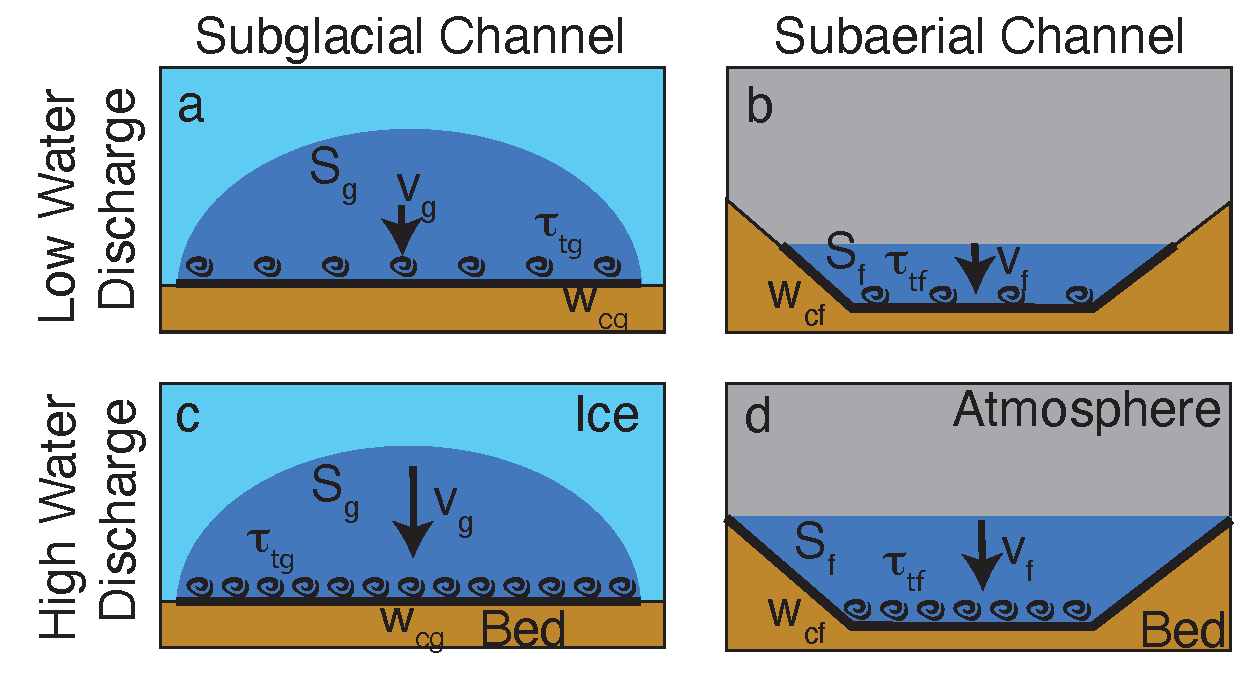
\includegraphics[width=0.65\linewidth]{Cartoon.pdf}
      \caption{Cartoon of the situation with various parameters. Velocity $v_g$ and $v_f$ magnitude are shown by arrow length and marks at the channel boundary. $S_g$ and $S_f$ represent the cross-sectional area in glacial and fluvial channels.  Note that in the fluvial channel parameterization, rectangular channel shapes are implemented (Section~\ref{sect:fluv}).} 
      \label{fig:cartoon}
    \end{figure}
  \end{center}
  
  \section{Methodology}
  \label{sect:meth}
  This section contains the relationships between water discharge, subglacial water velocity, and channel geometry in both fluvial and subglacial channels.
  Because sediment transport largely depends on shear stress \citep{shields1936}, both parameterizations calculated this value and integrate  it across the channel bed.
  The parameterizations evaluate shear stress, as opposed to sediment transport capacity, as shear stress omits a grain size parameter and the choice of a sediment transport relationship \citep{shields1936}.

  \ian{check units on fluvial channel factor}
  \begin{table}[H]
    \centering
    \caption{Variables, parameters, and constants }
    \begin{tabular}{ l  c  c c }
      Name &Symbol&  Value&Units \\ \hline
      \textbf{Variables}  & & & \\
      Channel hydraulic diameter (glacier, fluvial) &  $D_{hg},\,D_{hf}$&  & $\mathrm{m}$     \\
      Width of channel floor (glacial, fluvial) & $w_{cg},w_{cf}$&  & $\mathrm{m}$     \\
      Channel cross-sectional area (glacier, fluvial) &  $S_g, S_f$& & $\mathrm{m^2}$     \\
      Water discharge (instantaneous) & $Q_w$& & $\mathrm{m^{3}\,s^{-1}}$ \\
      Representative water discharge & $Q_{w}^*$& & $\mathrm{m^{3}\,s^{-1}}$ \\
      % Gradient of hydraulic potential (glacier) &$\Psi$ & & $\mathrm{Pa\, m^{-1}}$\\
      Representative hydraulic gradient  &$\Psi^*$ & & $\mathrm{Pa\, m^{-1}}$\\
      Water velocity (glacier, fluvial)  & $v_g,\,v_{f}$& & $\mathrm{m\,s^{-1}}$ \\
      Shear stress (glacier, fluvial) & $\tau_g,\,\tau_f$&& $\mathrm{Pa \, m^{-1}}$ \\
      Width-integrated shear-stress (glacier, fluvial) & $\tau_{tg},\, \tau_{tf}$&& $\mathrm{Pa \, m^{-1}}$ \\
      Reynolds number &$R_e$& & $\mathrm{(-)}$\\
      Variable &$\Gamma$&&$\mathrm{(-)}$\\
      Variability of a variable ($\Gamma$) &$\chi$& &$\mathrm{(-)}$\\
           &&&\\
      
      \textbf{Parameters and Constants}  & & &\\
      Gravitational constant&$g$& $-9.81$&$\mathrm{m\,s^{-2}}$\\
      Density of water & $\rho_w$& $1000$ & $\mathrm{kg\,m^{-3}}$ \\
      Density of ice & $\rho_i$& $900$ & $\mathrm{kg\,m^{-3}}$ \\
      Kinematic viscosity of water &$\nu$& $10^{-4}$& $\mathrm{m^2\,s^{-1}}$\\
      Hooke angle of channel & $\beta$ & $\frac{\pi}{2}$ & \unit{rad}\\
      Flotation fraction & $f_f$&$0.7$& $\mathrm{(-)}$\\
      Friction factor (glacier) & $f_r$ & $4$ & $\mathrm{(-)}$ \\
      Friction factor (fluvial) & $f_p$ & $3$ & $\mathrm{(-)}$\\
      Gradient of glacier surface & $\frac{\partial z_{sg}}{\partial x}$ &$0.25$& $\mathrm{(-)}$\\
      Gradient of channel bed (fluvial) &$\frac{\partial z_c}{\partial x}$ &$0.05$& $\mathrm{(-)}$\\
      Fluvial channel factor & $k$ &$3$ & $\mathrm{m^{-2}\, s}$\\
      Channel geometry exponent &$e$& $\frac{1}{2}$&$\mathrm{(-)}$ \\
      \hline
    \end{tabular}
    \label{table:vpm}
  \end{table}
  
  \subsection{Subglacial channel  parameterization}
  \label{sect:sub_mode}
  To parameterize the shear stress of water flowing across sediments below a glacier, the subglacial channel parameterization evaluates the channel geometry and the velocity of the flowing water. 
  To accomplish this, the hydraulics parameterization presented in \citet{delaney2019} is used.
  The parameterization uses the assumption that the water is transported through subglacial channels \citep[Figure~\ref{fig:cartoon}; ][]{rothlisberger1972}, and that a channel and geometry will respond to a representative water discharge over a certain time period $Q_{w}^*$, using the Darcy-Weisbach formulation for water-flow through a pipe to describe this relationship \citep[e.g.][]{rothlisberger1972,clarke2003,werder2013}.
  Here, it is assumed that the hydraulic diameter of the subglacial channel, $D_h$, responds to a representative water discharge, $Q_{w}^*$, and a representative gradient of the hydraulic potential, $\Psi^*$:
  \begin{linenomath*}
    \begin{equation}
      \label{eq:DW}
      D_h = \big(s\, f_r\,\rho_w\, \frac{Q_w^{*\,2}}{\Psi^*}\big)^{\frac{1}{5}}~~.
    \end{equation}
  \end{linenomath*}
  % 
  The representative hydraulic gradient is based upon the pressurized flow in Equation~\ref{eq:DW},
  \begin{equation}
    \label{eq:psi}
    \Psi^*= f_f \,  \rho_i \, g (\frac{\partial  z_{sg}}{\partial x} - \frac{\partial z_c}{\partial x}) +  \rho_i \, g \, \frac{\partial z_c}{\partial x},
  \end{equation}
  % 
  \noindent
  where, $f_f$ is the flotation fraction, $\rho_i$ is density of ice $\frac{\partial z_{sg}}{\partial x}$ is the surface slope of the glacier and $\frac{\partial z_c}{\partial x}$ is the glacier bed slope.
  
  In Equation~\ref{eq:DW}, $f_r$ is the Darcy-Weisbach friction factor and $\rho_w$ is the density of water (Table \ref{table:vpm}). $s$ is a factor accounting for channel geometry \citep{hooke1990}, calculated as:
  \begin{equation}
    \label{eq:Hf}
    s = \frac{2\,(\beta -\sin \beta)^2}{(\frac{\beta}{2}\,+\,\sin \frac{\beta}{2})^4},
  \end{equation}
  where $\beta$ is the central angle of the circular segment that comprises the channel (the so-called Hooke angle).
  Smaller values of $\beta$ result in shallow, wide channels. $\beta =\pi$ corresponds to a semi-circle.
  The width of the flat channel floor $w_c$ is given by
  \begin{equation}
    \label{eq:dh2wc}
    w_{cg} = 2  \sin \frac{\beta}{2} \sqrt{\frac{2\, S}{\beta -\sin \beta}},
  \end{equation}
  % 
  where $S$ is the cross-sectional area of the channel given by
  \begin{equation}
    \label{eq:dh2S}
    S_g =  \frac{D_h^2}{2}~ \frac{\Big(\frac{\beta}{2} \,+ \, \sin \frac{\beta}{2}\Big)^2  }{\beta\,-\,\sin \beta}.
  \end{equation}
  
  The shear stress, $\tau$, between the water and the channel bed is determined through the Darcy-Weisbach formulation
  \begin{equation}
    \label{eq:tau}
    \tau_g=\frac{1}{8}\,f_r\,\rho_w\,v_g^2,
  \end{equation}
  % 
  where $v_g = \frac{Q_w}{S_g}$ is the water velocity.
  Here, $Q_w$ represents the instantaneous water discharge, not used to evaluate the hydraulic gradient of the channel in Equation~\ref{eq:DW}.
  The channel size is usually not in equilibrium with the quantity of water flowing through it.
  With this formulation, the processes in an R-channel can be represented algebraically \citep{delaney2019}.
  
  For purposes discussed below, we evaluate the width integrated shear stress as $\tau_{tg}=w_{cg}\,\tau_g $.
  
  \subsection{Fluvial channel  parameterization}
  \label{sect:fluv}
  
  The fluvial channel parameterization implements the hydraulics parameterization presented in \citet{tucker1997}.
  Here, the assuming the conservation of mass, sufficiently wide channels so that the hydraulic radius is consistent with flow depth, uniform flow, and the Darcy-Weisbach relationship,
  the shear stress $\tau_f$ at the river bed is represented as
  \begin{linenomath*}
    \begin{equation}
      \label{eq:DW_tau}
      \tau_f=\frac{\rho_w\,g^{\frac{2}{3}}\,f_p^{\frac{1}{3}}}{2}\, \Big(\frac{Q_w}{w_{cf}} \Big)^{\frac{2}{3}} \,\frac{\partial z_c}{\partial x}^{\frac{2}{3}},
    \end{equation}
  \end{linenomath*}
  where $\frac{\partial z_c}{\partial x}$ is the channel slope, and $f_p$ is the friction factor for fluvial systems.
  Channel width $w_{cf}$ is 
  \begin{equation}
    \label{eq:wcf}
    w_{cf} = k \, Q_w^e,
  \end{equation}
  % 
  where $k$ is a constant and $e$ is an exponent commonly equal to $\frac{1}{2}$ \citep{leopold1953}. Cross-sectional area is 
  \begin{equation}
    \label{eq:Sf}
    S_f= \frac{Q_w}{v_f}.
  \end{equation}
  As in Section~\ref{sect:sub_mode}, the width integrated shear stress is $\tau_{tf}=w_{cf}\,\tau_f$.
  Hydraulic diameter of the channel is given by $D_{hf} = \frac{4\,w_{cf}\,d}{2\,d+w_{cf}}$, with flow depth $d$ determined from knowledge of $S_f$ and $w_{cf}$ in a rectangular channel.
  
  \subsection{Implementation}
  
  The formulation for the glacial system above requires inputs of the hydraulic gradient, water discharge, representative water discharge, Hooke angle $\beta$ \citep{hooke1990}, and friction factor $f_r$.
  Values of $\beta$ and $f_r$ are chosen so that they produce reasonable values of water velocity, in accordance with available measurements through dye-tracing \citep[Section~\ref{sect:sub_mode}, Figure~\ref{fig:model_outs}; e.g.][]{werder2010}.
  
  In the fluvial system, the water is not pressurized, so only the bed slope is needed. Friction factor $f_f$ and channel shape factor $k$ are assigned (Section~\ref{sect:fluv}).
  
  The Reynolds number $R_e$ is given as 
  \begin{equation}
    \label{eq:re}
    R_e\,=\, v \,\frac{D_h}{\nu},
  \end{equation}
  % 
  \noindent where $\nu$ is the kinematic viscosity of water, and  $v$ is velocity of water, $v_g$ or $v_f$.
  
  The variance $ \chi$ of a variable $\Gamma$ is given by 
  \begin{equation}
    \label{eq:var}
    \chi(\Gamma) \,=\, 1 - \frac{\mathrm{min}(\Gamma)}{\mathrm{max}(\Gamma)}\,\,.
  \end{equation}
  % 
  \noindent Below we examine variables, $\Gamma$, as water discharge ($Q_w$) water velocity ($v$, $v_f$), shear stress ($\tau$, $\tau_f$), and integrated shear stress ($\tau_t$, $\tau_{tf}$).
  
  
  \section{Results}
  First, the subglacial hydraulics parameterization is applied to a representative water discharge ($Q_w^*$; Equation~\ref{eq:DW}) of $12$\,\unit{m}$^{3}$\,\unit{s}$^{-1}$.
  Both parameterizations are forced with a water discharge ($Q_w$) varying between $8$ and $16$ \,\unit{m}$^{3}$\,\unit{s}$^{-1}$, to represent a range of sediment transport conditions, for instance over diurnal fluctuation in water discharge. The fluvial channel width factor $k$ is $3$\,\unit{m}$^{2}$\,\unit{s}$^{-1}$, and the Hooke angle $\beta$ is $\frac{\pi}{2}$.
  
  \begin{center}
    \begin{figure}[H]
      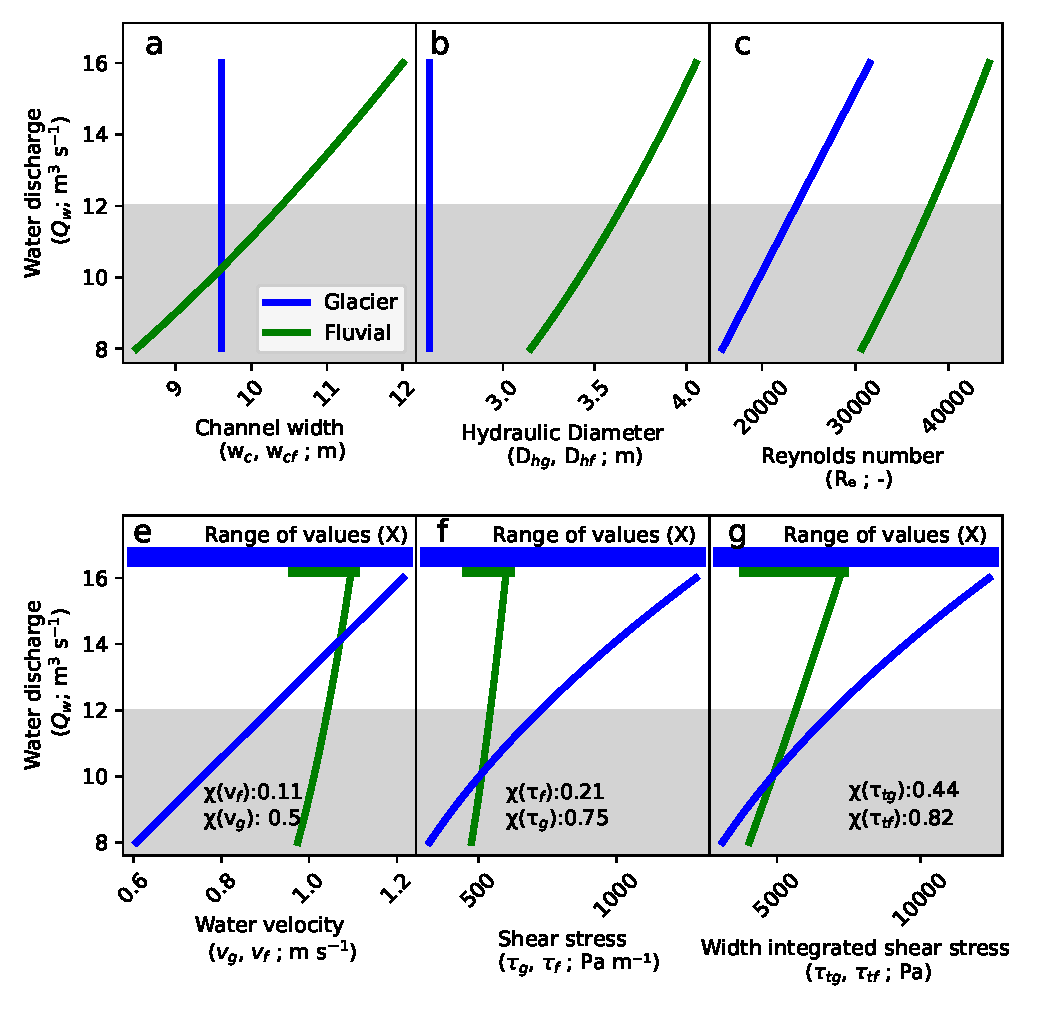
\includegraphics[width=0.7\linewidth]{model_outputs.pdf}
      \caption{Response of channel width (a), hydraulic diameter (b),  Reynolds number  (c),  water velocity (d), shear-stress (e), and width-integrated shear-stress (f)  to different water discharge values. The glacial system is in blue and the fluvial system is in green.  Horizontal bars in d, e, and f represent the range of values in the  output. Gray space represents water discharge below the mean value. }
      \label{fig:model_outs}
    \end{figure}
  \end{center}
  
  Across the hydrological forcing, variable water discharge results in a substantial increase in the range of water velocities in the glacial system compared to the fluvial system (Figure~\ref{fig:model_outs}).
  While water velocity in the glacier system varies by  $0.5$ (Equation~\ref{eq:var}) over the discharge values, in the fluvial system the water velocity only varies by $0.11$.
  Similarly, shear stress at the glacier bed varies by $0.75$ across the range of water discharge values, whereas shear stress across the fluvial system varies by roughly $0.21$. This increased variability  in shear stress between the two systems occurs as the water velocity is raised to the power of $2$ in Equation~\ref{eq:tau}. 
  
  Changing channel geometry accommodates evolving water discharge in the fluvial system (Equation~\ref{eq:wcf}), whereas in the subglacial case, increased water flux can only be accommodated by an increase in velocity (Equation~\ref{eq:DW}).
  The range of values between width-integrated shear stress in the fluvial system increases to $0.44$, whereas, variability in the glacial system lies at $0.83$ (Figure~\ref{fig:range}).
  Indeed, the relative  difference in width-integrated shear stress is less between the fluvial and glacier cases, compared to the water velocity and shear stress outputs.
  The reduced variability in width-integrated shear stress results from the additional width across the fluvial channel that accommodates a portion of the sediment transport capacity.
  
  Next, the parameterizations are run $25,000$ times with randomly selected channel geometries ($k=(2,6)$, $\beta=(\frac{\pi}{10},\pi)$), friction factors ($f_i=(0.001,20)$, $f_p=(0.001,20)$) and water discharges (maximum and minimum values selected between $5$ to $500$ \,\mmma). $Q_w^*$ in Equation ~\ref{eq:DW} is determined as the midpoint in the water discharge range. Parameter combinations are only selected if their maximum and minimum velocities are between $0.2$ and $3$\,\unit{m}\,\unit{s}$^{-1}$, resulting in roughly $10,600$ adequate parameter combinations. 
  
  
  \begin{center}
    \begin{figure}[H]
      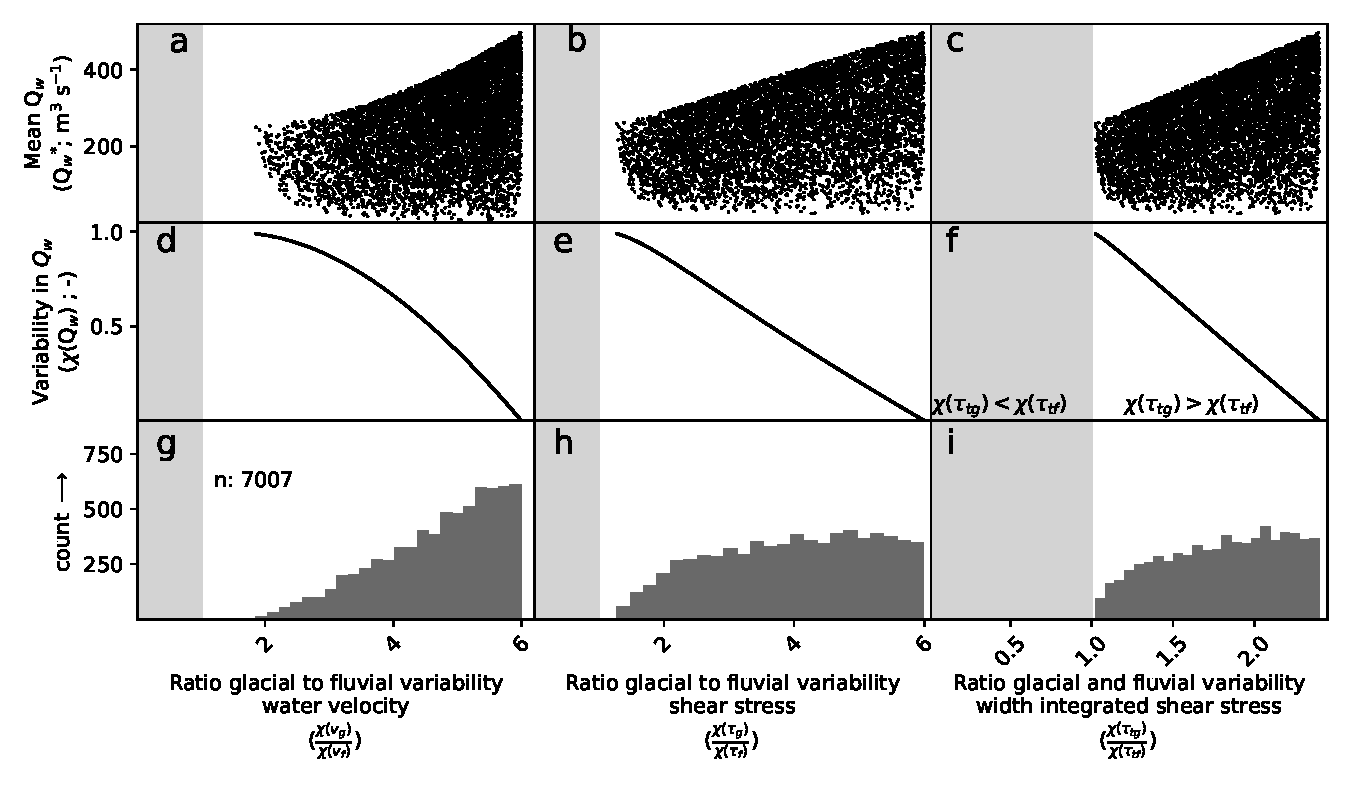
\includegraphics[width=0.7\linewidth]{multi_run.pdf}
      \caption{Ratio of range of a variable $\Gamma$ for glacial and fluvial systems for water velocity  (a), shear-stress (b), and  width-integrated shear-stress (c) in response to mean water discharge,
        Range  $\chi$ for each variable is given in Equation~\ref{eq:var}. Values greater (less) than $1$ shown in white (gray) are parameter combinations that vary more in a subglacial (fluvial) system. Plots (d-f) show the response of variable $\Gamma$ to the variability in water discharge ($\chi(Q_w)$) in the parameter combination. 
        Histograms (g-i) show the frequency of relative variations across variables in the parameterization.}
      \label{fig:range}
    \end{figure}
  \end{center}
  
  Across the accepted model runs, variability in water velocity and shear stress remains substantially higher across the subglacial model compared to fluvial ones (Figure~\ref{fig:range}).
  Water velocity, shear stress, and width-integrated shear stress all have a variability ratio ($\frac{\chi(\Gamma_{g})}{\chi(\Gamma_f)}$) greater than $1$ in the subglacial  system compared to fluvial one (Figure~S1).
  
  The minimum ratio of  water velocity, $\frac{\chi(v_{g})}{\chi(v_{f})}$, and shear-stress, $\frac{\chi(\tau_{g})}{\chi(\tau_{f})}$, is around $2$, showing that these factors are substantially more variable in subglacial channels compared to fluvial ones.
  The width integrated shear stress, $\frac{\chi(\tau_{tg})}{\chi( \tau_{tf})}$, spans between $1.02$ and $2.4$ because changing channel width accommodates the reduced shear stress in the fluvial system.
  No runs experienced width integrated shear stress, $\frac{\chi(\tau_{tg})}{\chi( \tau_{tf})}$, less than $1$.
  
  Runs with the smallest variability in discharge ($\chi(Q_w)$) have the greatest variability in water velocity, shear stress, and width-integrated shear stress in subglacial systems compared to fluvial ones (Figure~\ref{fig:range} and S1).
  Yet, the greatest difference in the two systems at the smallest variations of water discharge still results in greater variability in the subglacial system compared to the fluvial one (Figure S1). 

  
  \section{Discussion}
  \subsection{Assumptions}
  
  The direct comparison between the systems remains difficult as they have with different hydraulic potentials, and the response of channel width to water discharge varies considerably based on the values chosen for $\beta$ and $k$.
  
  The subglacial parameterization assumes that subglacial water is pressurized, which is a commonly held assumption in subglacial hydrology, though observations suggest that this may not always be the case \citep[e.g.][]{gimbert2016}.
  While the subglacial channel geometry need not be in a steady state for the water to remain pressurized, the subglacial parameterization assumes that the channel geometry must vary minimally over the timescales of varying  water discharge \citep[e.g.][]{nanni2020}.
  
  In R-channel formulations, peaks in the hydrograph could cause additional opening of the conduit due to pressure melt, thus causing a decrease in velocity compared to the results here \citep{rothlisberger1972}.
  A similar effect could occur with creep closure of the subglacial channel at the hydrograph minima.
  Additionally, at high water pressures, glacier uplift and bed separation \citep{andrews2014} might slightly modify the width of the subglacial channel. 

  Both subglacial and fluvial parameterizations here assume that the distribution of velocity and shear stress of water across the channel bed is homogeneous (Section~\ref{sect:sub_mode}~and~\ref{sect:fluv}). 
  The fluvial parameterization assumes that sediment is transported across all channel widths, as opposed to bankfull width when much sediment transport occurs \citep{wolman1960}.
  As a result, the variability in the fluvial system across the range of discharge values could be underestimated in the parameterization (Figure~\ref{fig:range}).
  
  
  
  \subsection{Geomorphic Implications}
  \label{sect:GI}
  The consistent relationship between water discharge variability and relative variability of the water velocity, shear stress, and width-integrated shear stress results from the fixed geometry in the glacier system and variable geometry in the fluvial system as they respond to changes in water discharge (Equations~\ref{eq:tau} and \ref{eq:Sf}).
  Increased variability in sediment transport capacity with respect to discharge has several implications for sediment transport in subglacial systems compared to fluvial ones.
  Shear stress is scaled to the $\frac{3}{2}$ power  and relies on shear stress exceeding a threshold in sediment transport relationships  such as \citet{meyer1948}.
  In the total sediment transport relationship \citet{engelund1967}, the shear stress is scaled to $\frac{5}{2}$ power.
  In both cases, the exponent greater than $1$ magnifies the variability in sediment transport beyond the highly variable shear stress and width-integrated shear stress described above in subglacial environments (Figure~\ref{fig:model_outs}\, b and d; Figure~S1).

  \subsubsection{Sediment transport below glaciers and at their margins}
  
  The response of sediment discharge caused by the greater variability in sediment transport in subglacial channels will be greatest in completely transport-limited regimes \citep[e.g.][]{kasmalkar2019}.
  In supply-limited systems, the changing sediment transport capacity (Figure~\ref{fig:model_outs}) would have a minimal effect on sediment discharge due to the absence of sediment available for transport \citep{delaney2019}.
  Yet, reaching the threshold of motion for sediment more frequently may result in additional sediment transport and the tendency for glaciers to transport sediment in a supply-limited regime \citep[e.g.][]{herman2015}.
  
  The effect of pressurized channel flow could be most pronounced during precipitation or flood events when subglacial conduits have not adapted to the water discharge flowing through them, resulting in a very large increase in sediment transport capacity and discharge \citep[e.g.][]{cowan1988,delaney2019}.
  Increased sediment discharge may result from changes to sediment access below the glacier, yet rapid increases in water velocity from water flowing through a small conduit, not conditioned by the amount of water flow, will cause a large increase in sediment transport capacity (Section~\ref{sect:sub_mode}).
  
  Increased variability in sediment transport also impacts sediment export from glacier margins into proglacial areas \citep[e.g.][]{delaney2017,perolo2018}.
  Here, in the transition to open-channel flow as the water leaves the glacier, velocities at the highest water discharges could generally decrease (Figure~\ref{fig:model_outs}, blue and green horizontal bars), potentially resulting in sediment deposition once sediment enters the proglacial area.
  Note that the transition from pressurized to open channel flow could occur above the glacier's terminus, when cavity closure rates are reduced and water can flow freely \citep{egli2021b}, resulting in intermittent deposition and remobilization of sediment below the glacier terminus \citep{perolo2018}.
  
  In large catchments and further downstream of proglacial margins, water discharge is generally less variable than at the tops of catchments, where glaciers lie \citep[c.f.][]{costa2017,vanas2017,delaney2018,hasholt2018}.
  Here, external hydrological factors further downstream of glaciers could result in smaller variations in sediment transport capacity in many fluvial systems compared to subglacial ones.
  The parameterization here shows that the smallest variability in water discharge has the largest difference in relative variability from subglacial to proglacial systems (Figure~\ref{fig:range}\, d,\,e,\,f), while the variability in the subglacial system remains higher (Figure~S1).
  Therefore, at locations such as the Greenland Ice Sheet, with smaller diurnal variations in water discharge compared to many alpine catchments \citep[c.f.][]{delaney2018,hasholt2018}, the variability in sediment transport capacity in the transition from the ice sheet to the proglacial river could be more dramatic than alpine systems as water leaves the glacier and moves downstream.
  Thus the disparity in sediment transport capacity between the subglacial and fluvial systems could be most pronounced in these catchments, potentially resulting in temporally mismatched periods between when glaciers introduce sediment to these river systems  and when the river mobilizes it (Figures~\ref{fig:range}~ and~\ref{fig:model_outs}).
  
  
  \subsubsection{Records of sediment discharge  from glaciers}
  
  Large variations in sediment transport capacity below glaciers may result in sediment mobilization and deposition processes in close spatial and temporal proximity to each other below the glacier \citep{gimbert2016,perolo2018}, in response to both evolving channel geometry and water discharge with accumulating with melt down-glacier \citep{beaud2018,delaney2019}.
  Increasing variability in sediment transport down-glacier is likely because of spatial discontinuities in sediment availability, increasing water discharge down the glacier, and the transport times of subglacial sediment \citep{williams1989,delaney2019}.
  The rapid increase and decreases in sediment transport capacity over a diurnal cycle in a subglacial system, for instance, compounds the variability already present in fluvial systems \citep{williams1989,jerolmack2010}.
  As a result, variations in sediment transport capacity could be responsible for the fluctuations in sediment discharge (``flushings'') from glaciers that are not attributed to variations in water discharge \citep[e.g.][]{richards2003,swift2021}, but could be the result of reduced conduit size and therefore increased sediment transport capacity.

  Additional processes and erosional hiatuses may further complicate signals of sediment discharge from glaciers in response to climate, compared to fluvial systems \citep{jansson2005,ganti2016}. 
  For instance, if a glacier expels sediment in a transport-limited regime, the pressurized nature of subglacial water flow means sediment discharge capacity responds to the thickness of the ice, controlling the closure of the channel, and the surface slope of the glacier, controlling water velocity, in addition to water discharge \citep[Section~\ref{sect:sub_mode}; ] []{rothlisberger1972,shreve1972}.
  Conversely, sediment transport in most fluvial systems increases with water discharge and bed slope, with the bed slope, probably being more stable over long time periods \citep[Section~\ref{sect:fluv}; e.g.][]{muller1968,whipple1999,wong2006}. 
  Furthermore, if the glacier is in a supply-limited case, the sediment discharge record will also represent additional processes of sliding  \citep{herman2015,seguinot2021}, adding additional processes represented in the sediment discharge signal \citep{delaney2019}.
  
  Records of sediment discharge have been used to establish the relationship, or lack thereof, between sediment discharge and climate in glacial systems \citep[e.g.][]{koppes2009a,willenbring2016,mariotti2021}.
  The variability in subglacial sediment transport capacity presented here applies most generally to short-time scales responsible for the size of subglacial channels.
  Yet, identifying climatic signals in sediment transport from transport-limited glaciers may require higher thresholds of climatic perturbation compared to fluvial systems \citep{tofelde2021}, given the potential amount of additional noise \citep{castletort2003,jerolmack2010,romans2016}.
  For instance, sediment discharge records from two glaciers in the Swiss Alps show that $40$ to $50$\% of a season's sediment discharge occurs when water discharge is below the $75^{\mathrm{th}}$ quantile of the season \citep{delaney2018}, possibly because sediment transport capacity relies on the size of the glacier conduit, in addition to water discharge (Section~\ref{sect:sub_mode}).
  This suggests that a larger climate perturbation might be needed to significantly alter the sediment discharge capacity from the glaciers compared to fluvial systems, to overcome the increased variability in sediment transport capacity.


  \section{Conclusions}
  
  Application of parameterizations for subglacial and fluvial water flow shows that variable processes occur in sediment transport capacity's response to water discharge, due to their fixed and variable channel geometry, respectively.
  Results show that the impact of variable water discharge on water velocity and shear stress, first-order controls on sediment mobilization, is much higher in subglacial channels than in fluvial ones.
  The variability in shear stress is reduced when the evolving channel width is accounted for in fluvial systems.
  Even so, variability in shear stress across a channel's width is still higher in subglacial channels, compared to fluvial ones.
  
  These different characteristics between glacial and fluvial channels show that records of sediment transport downstream of glaciers capture multiple fluvial processes together.
  Such processes might be particularly relevant at glacier margins, where water transitions from pressurized subglacial flow to open-channel flow.
  The inconsistent response of sediment transport in subglacial and fluvial systems to changing water discharge could add noise to sediment transport signals between the systems.
  In addition, the subglacial parameterization shows that variations in sediment transport capacity in glacier systems respond to a large number of factors such as channel size, ice thickness, and glacier surface slope, which may react to climate forcing differently than water discharge alone. 
  The differences in fluvial and subglacial channels' response to changing water discharge should be considered when examining sediment transport processes in glacierized catchments.
  
  \section{Acknowledgments}
  
  I was funded by SNSF Project No. PZ00P2\_202024.
  The julia code used herein is included in the supplementary material.
  
  
\end{spacing}

\bibliographystyle{apalike}
\bibliography{Paperlib.bib}


\section{Supplement}

\begin{center}
  \begin{figure}[H]
    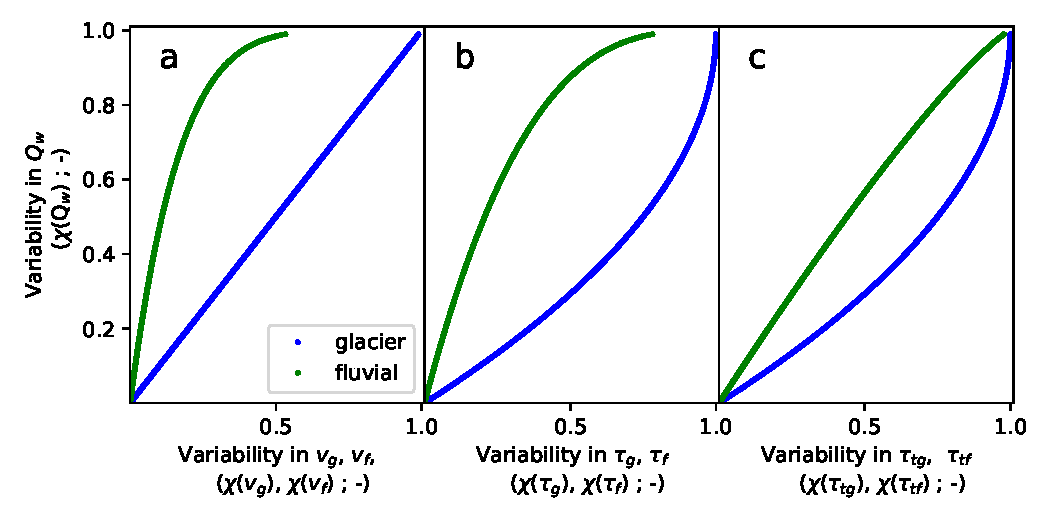
\includegraphics[width=0.7\linewidth]{multi_run_vars.pdf}
    \caption{Variability $\chi$ in velocity ($v_g$, $v_f$; a) shear stress ($\tau_g$, $\tau_f$; b) and width-integrated shear stress ($\tau_{tg}$, $\tau_{tf}$; c)  in glacial and fluvial systems. }
    \label{fig:gammas}
  \end{figure}
\end{center}




\end{document}

%%% Local Variables:
%%% mode: latex
%%% TeX-master: t
%%% End:

% LocalWords:  pre todo phillips CVODE decadal refreezing Mauro eq%  LocalWords:  dQs
% LocalWords:  dx ms ca DF Hm meltwater Griessee gridded ehrbar ng
% LocalWords:  koppes costa bendixen delaney herman hallet creyts ian
% LocalWords:  farinotti stott rickenman delaney2019 plagerized
% LocalWords:  fischer zekollari clarke raymond larour delaneyinprep
% LocalWords:  guillon exner wolman engelund Weisbach

As a result, the parameterization here is most relevant for relatively wide rivers, where channel width evolves greatly with water discharge (Equation~\ref{eq:wcf}).
% This is probably the case in many proglacial rivers and glacierized catchments where the divergent behavior of subglacial and fluvial channels is most relevant (Figure~\ref{sect:GI}) \ian{Find reference about the geometry of proglacial river}.


Qbs_out Qws_out